% =====================================================================
% Component Diagram: CleanTest-Agent module dependencies
%
% Standalone, paper-grade reproduction of Figure "Component Diagram:
% Module Dependencies" in report/main.tex (Section 6, System Design).
% Source nodes, positions, and dependency edges are byte-identical with
% the manuscript so the exported PDF / PNG / SVG can be cited as the
% same figure.
%
% Build:
%     pdflatex component-diagram.tex          % default: paper colours
%     pdflatex "\def\BW{1}% =====================================================================
% Component Diagram: CleanTest-Agent module dependencies
%
% Standalone, paper-grade reproduction of Figure "Component Diagram:
% Module Dependencies" in report/main.tex (Section 6, System Design).
% Source nodes, positions, and dependency edges are byte-identical with
% the manuscript so the exported PDF / PNG / SVG can be cited as the
% same figure.
%
% Build:
%     pdflatex component-diagram.tex          % default: paper colours
%     pdflatex "\def\BW{1}% =====================================================================
% Component Diagram: CleanTest-Agent module dependencies
%
% Standalone, paper-grade reproduction of Figure "Component Diagram:
% Module Dependencies" in report/main.tex (Section 6, System Design).
% Source nodes, positions, and dependency edges are byte-identical with
% the manuscript so the exported PDF / PNG / SVG can be cited as the
% same figure.
%
% Build:
%     pdflatex component-diagram.tex          % default: paper colours
%     pdflatex "\def\BW{1}% =====================================================================
% Component Diagram: CleanTest-Agent module dependencies
%
% Standalone, paper-grade reproduction of Figure "Component Diagram:
% Module Dependencies" in report/main.tex (Section 6, System Design).
% Source nodes, positions, and dependency edges are byte-identical with
% the manuscript so the exported PDF / PNG / SVG can be cited as the
% same figure.
%
% Build:
%     pdflatex component-diagram.tex          % default: paper colours
%     pdflatex "\def\BW{1}\input{component-diagram}"   % grayscale
%
% Or use the wrapper script:
%     ./build-figures.sh
%
% Notes on classfile choice:
%     We use `article` + `geometry` (everywhere available) instead of
%     `standalone` (requires `texlive-pictures`, not in BasicTeX) so the
%     figure builds on a stripped-down TeX install. The generated PDF is
%     subsequently cropped to the figure bounding box by `pdfcrop`,
%     yielding the same artefact a `standalone` build would.
% =====================================================================
\documentclass[11pt]{article}

\usepackage[paperwidth=22cm,paperheight=8.8cm,margin=4mm]{geometry}
\usepackage{lmodern}            % Computer Modern at scalable Type-1
\usepackage[T1]{fontenc}
\usepackage{tikz}
\usetikzlibrary{shapes,arrows.meta,positioning,calc}
\pagestyle{empty}

% ---------------------------------------------------------------------
% \BW = 1 switches to a print-safe grayscale palette. Default is the
% colour palette used in the paper (orange skills / blue core / grey
% libraries), which is the convention this figure has in the report.
% ---------------------------------------------------------------------
\providecommand{\BW}{0}

\ifnum\BW=1
  \definecolor{cSkill}{gray}{0.92}
  \definecolor{cCore} {gray}{0.85}
  \definecolor{cLib}  {gray}{0.78}
\else
  \definecolor{cSkill}{RGB}{255,237,213}   % orange!10
  \definecolor{cCore} {RGB}{219,234,254}   % blue!10
  \definecolor{cLib}  {RGB}{229,231,235}   % gray!10
\fi

\begin{document}
\centering
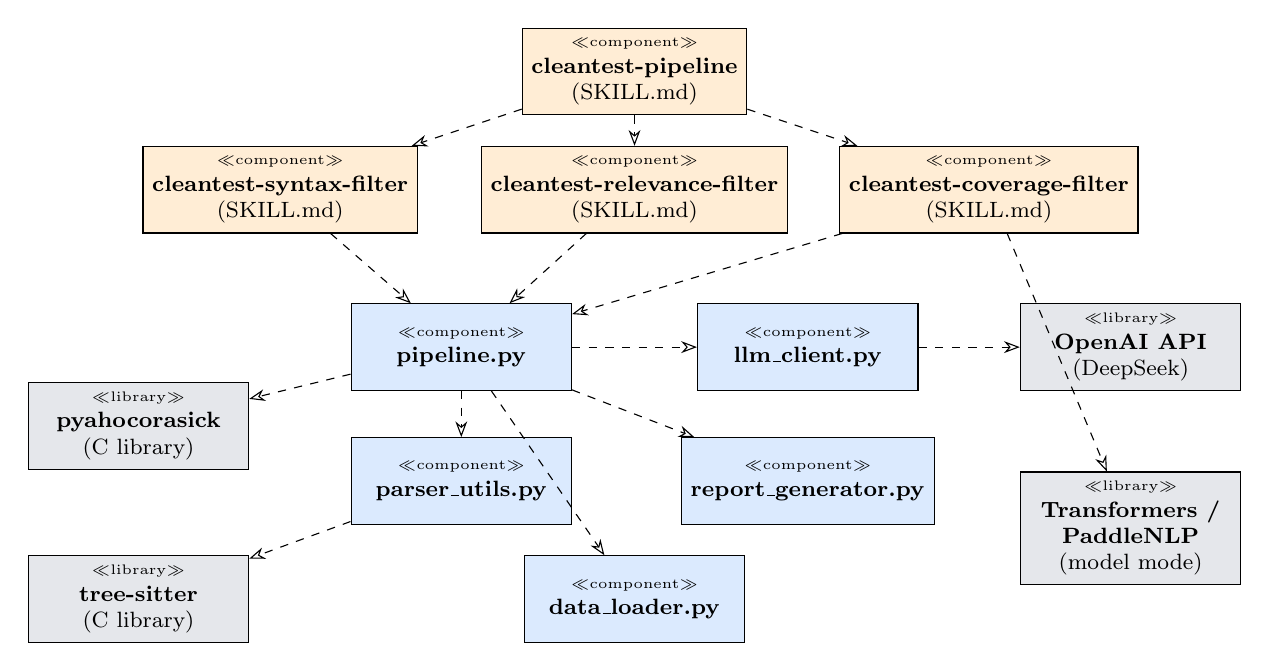
\begin{tikzpicture}[
    node distance=0.8cm,
    comp/.style={rectangle, draw, minimum width=2.8cm, minimum height=1.1cm,
                 align=center, font=\footnotesize, line width=0.4pt},
    % UML 2.5.1 §7.8.4 Dependency: dashed line with an open V-shaped
    % stick arrowhead (NOT a triangular arrowhead, which denotes
    % generalization or realization).
    dep/.style={-{Stealth[length=2mm,open]}, dashed, line width=0.4pt},
]
% --- Skills layer (UML 2.5.1 components are stereotyped <<component>>).
\node[comp, fill=cSkill] (pipe) at (0,4)
    {{\tiny$\ll$component$\gg$}\\\textbf{cleantest-pipeline}\\(SKILL.md)};
\node[comp, fill=cSkill] (sf) at (-4.5,2.5)
    {{\tiny$\ll$component$\gg$}\\\textbf{cleantest-syntax-filter}\\(SKILL.md)};
\node[comp, fill=cSkill] (rf) at (0,2.5)
    {{\tiny$\ll$component$\gg$}\\\textbf{cleantest-relevance-filter}\\(SKILL.md)};
\node[comp, fill=cSkill] (cf) at (4.5,2.5)
    {{\tiny$\ll$component$\gg$}\\\textbf{cleantest-coverage-filter}\\(SKILL.md)};

% --- Core library
\node[comp, fill=cCore] (pipeline) at (-2.2,0.5)
    {{\tiny$\ll$component$\gg$}\\\textbf{pipeline.py}};
\node[comp, fill=cCore] (parser) at (-2.2,-1.2)
    {{\tiny$\ll$component$\gg$}\\\textbf{parser\_utils.py}};
\node[comp, fill=cCore] (llm) at (2.2,0.5)
    {{\tiny$\ll$component$\gg$}\\\textbf{llm\_client.py}};
\node[comp, fill=cCore] (report) at (2.2,-1.2)
    {{\tiny$\ll$component$\gg$}\\\textbf{report\_generator.py}};
\node[comp, fill=cCore] (loader) at (0,-2.7)
    {{\tiny$\ll$component$\gg$}\\\textbf{data\_loader.py}};

% --- External libraries (custom <<library>> stereotype).
\node[comp, fill=cLib] (ts) at (-6.3,-2.7)
    {{\tiny$\ll$library$\gg$}\\\textbf{tree-sitter}\\(C library)};
\node[comp, fill=cLib] (aho) at (-6.3,-0.5)
    {{\tiny$\ll$library$\gg$}\\\textbf{pyahocorasick}\\(C library)};
\node[comp, fill=cLib] (api) at (6.3,0.5)
    {{\tiny$\ll$library$\gg$}\\\textbf{OpenAI API}\\(DeepSeek)};
\node[comp, fill=cLib] (tf) at (6.3,-1.8)
    {{\tiny$\ll$library$\gg$}\\\textbf{Transformers /}\\\textbf{PaddleNLP}\\(model mode)};

% --- Dependencies (UML 2.5.1 §7.8.4: dashed line + open V arrowhead).
\draw[dep] (pipe) -- (sf);
\draw[dep] (pipe) -- (rf);
\draw[dep] (pipe) -- (cf);
\draw[dep] (sf) -- (pipeline);
\draw[dep] (rf) -- (pipeline);
\draw[dep] (cf) -- (pipeline);
\draw[dep] (pipeline) -- (parser);
\draw[dep] (pipeline) -- (llm);
\draw[dep] (pipeline) -- (report);
\draw[dep] (pipeline) -- (loader);
\draw[dep] (parser) -- (ts);
\draw[dep] (pipeline) -- (aho);
\draw[dep] (llm) -- (api);
\draw[dep] (cf) -- (tf);
\end{tikzpicture}
\end{document}
"   % grayscale
%
% Or use the wrapper script:
%     ./build-figures.sh
%
% Notes on classfile choice:
%     We use `article` + `geometry` (everywhere available) instead of
%     `standalone` (requires `texlive-pictures`, not in BasicTeX) so the
%     figure builds on a stripped-down TeX install. The generated PDF is
%     subsequently cropped to the figure bounding box by `pdfcrop`,
%     yielding the same artefact a `standalone` build would.
% =====================================================================
\documentclass[11pt]{article}

\usepackage[paperwidth=22cm,paperheight=8.8cm,margin=4mm]{geometry}
\usepackage{lmodern}            % Computer Modern at scalable Type-1
\usepackage[T1]{fontenc}
\usepackage{tikz}
\usetikzlibrary{shapes,arrows.meta,positioning,calc}
\pagestyle{empty}

% ---------------------------------------------------------------------
% \BW = 1 switches to a print-safe grayscale palette. Default is the
% colour palette used in the paper (orange skills / blue core / grey
% libraries), which is the convention this figure has in the report.
% ---------------------------------------------------------------------
\providecommand{\BW}{0}

\ifnum\BW=1
  \definecolor{cSkill}{gray}{0.92}
  \definecolor{cCore} {gray}{0.85}
  \definecolor{cLib}  {gray}{0.78}
\else
  \definecolor{cSkill}{RGB}{255,237,213}   % orange!10
  \definecolor{cCore} {RGB}{219,234,254}   % blue!10
  \definecolor{cLib}  {RGB}{229,231,235}   % gray!10
\fi

\begin{document}
\centering
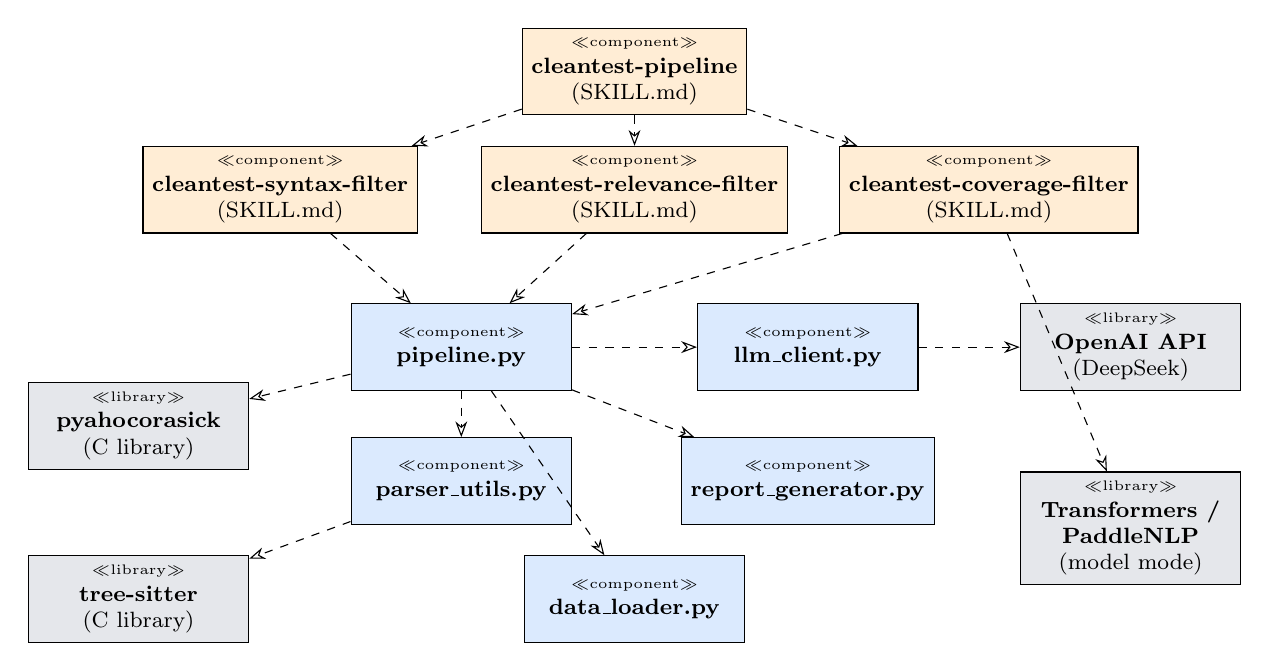
\begin{tikzpicture}[
    node distance=0.8cm,
    comp/.style={rectangle, draw, minimum width=2.8cm, minimum height=1.1cm,
                 align=center, font=\footnotesize, line width=0.4pt},
    % UML 2.5.1 §7.8.4 Dependency: dashed line with an open V-shaped
    % stick arrowhead (NOT a triangular arrowhead, which denotes
    % generalization or realization).
    dep/.style={-{Stealth[length=2mm,open]}, dashed, line width=0.4pt},
]
% --- Skills layer (UML 2.5.1 components are stereotyped <<component>>).
\node[comp, fill=cSkill] (pipe) at (0,4)
    {{\tiny$\ll$component$\gg$}\\\textbf{cleantest-pipeline}\\(SKILL.md)};
\node[comp, fill=cSkill] (sf) at (-4.5,2.5)
    {{\tiny$\ll$component$\gg$}\\\textbf{cleantest-syntax-filter}\\(SKILL.md)};
\node[comp, fill=cSkill] (rf) at (0,2.5)
    {{\tiny$\ll$component$\gg$}\\\textbf{cleantest-relevance-filter}\\(SKILL.md)};
\node[comp, fill=cSkill] (cf) at (4.5,2.5)
    {{\tiny$\ll$component$\gg$}\\\textbf{cleantest-coverage-filter}\\(SKILL.md)};

% --- Core library
\node[comp, fill=cCore] (pipeline) at (-2.2,0.5)
    {{\tiny$\ll$component$\gg$}\\\textbf{pipeline.py}};
\node[comp, fill=cCore] (parser) at (-2.2,-1.2)
    {{\tiny$\ll$component$\gg$}\\\textbf{parser\_utils.py}};
\node[comp, fill=cCore] (llm) at (2.2,0.5)
    {{\tiny$\ll$component$\gg$}\\\textbf{llm\_client.py}};
\node[comp, fill=cCore] (report) at (2.2,-1.2)
    {{\tiny$\ll$component$\gg$}\\\textbf{report\_generator.py}};
\node[comp, fill=cCore] (loader) at (0,-2.7)
    {{\tiny$\ll$component$\gg$}\\\textbf{data\_loader.py}};

% --- External libraries (custom <<library>> stereotype).
\node[comp, fill=cLib] (ts) at (-6.3,-2.7)
    {{\tiny$\ll$library$\gg$}\\\textbf{tree-sitter}\\(C library)};
\node[comp, fill=cLib] (aho) at (-6.3,-0.5)
    {{\tiny$\ll$library$\gg$}\\\textbf{pyahocorasick}\\(C library)};
\node[comp, fill=cLib] (api) at (6.3,0.5)
    {{\tiny$\ll$library$\gg$}\\\textbf{OpenAI API}\\(DeepSeek)};
\node[comp, fill=cLib] (tf) at (6.3,-1.8)
    {{\tiny$\ll$library$\gg$}\\\textbf{Transformers /}\\\textbf{PaddleNLP}\\(model mode)};

% --- Dependencies (UML 2.5.1 §7.8.4: dashed line + open V arrowhead).
\draw[dep] (pipe) -- (sf);
\draw[dep] (pipe) -- (rf);
\draw[dep] (pipe) -- (cf);
\draw[dep] (sf) -- (pipeline);
\draw[dep] (rf) -- (pipeline);
\draw[dep] (cf) -- (pipeline);
\draw[dep] (pipeline) -- (parser);
\draw[dep] (pipeline) -- (llm);
\draw[dep] (pipeline) -- (report);
\draw[dep] (pipeline) -- (loader);
\draw[dep] (parser) -- (ts);
\draw[dep] (pipeline) -- (aho);
\draw[dep] (llm) -- (api);
\draw[dep] (cf) -- (tf);
\end{tikzpicture}
\end{document}
"   % grayscale
%
% Or use the wrapper script:
%     ./build-figures.sh
%
% Notes on classfile choice:
%     We use `article` + `geometry` (everywhere available) instead of
%     `standalone` (requires `texlive-pictures`, not in BasicTeX) so the
%     figure builds on a stripped-down TeX install. The generated PDF is
%     subsequently cropped to the figure bounding box by `pdfcrop`,
%     yielding the same artefact a `standalone` build would.
% =====================================================================
\documentclass[11pt]{article}

\usepackage[paperwidth=22cm,paperheight=8.8cm,margin=4mm]{geometry}
\usepackage{lmodern}            % Computer Modern at scalable Type-1
\usepackage[T1]{fontenc}
\usepackage{tikz}
\usetikzlibrary{shapes,arrows.meta,positioning,calc}
\pagestyle{empty}

% ---------------------------------------------------------------------
% \BW = 1 switches to a print-safe grayscale palette. Default is the
% colour palette used in the paper (orange skills / blue core / grey
% libraries), which is the convention this figure has in the report.
% ---------------------------------------------------------------------
\providecommand{\BW}{0}

\ifnum\BW=1
  \definecolor{cSkill}{gray}{0.92}
  \definecolor{cCore} {gray}{0.85}
  \definecolor{cLib}  {gray}{0.78}
\else
  \definecolor{cSkill}{RGB}{255,237,213}   % orange!10
  \definecolor{cCore} {RGB}{219,234,254}   % blue!10
  \definecolor{cLib}  {RGB}{229,231,235}   % gray!10
\fi

\begin{document}
\centering
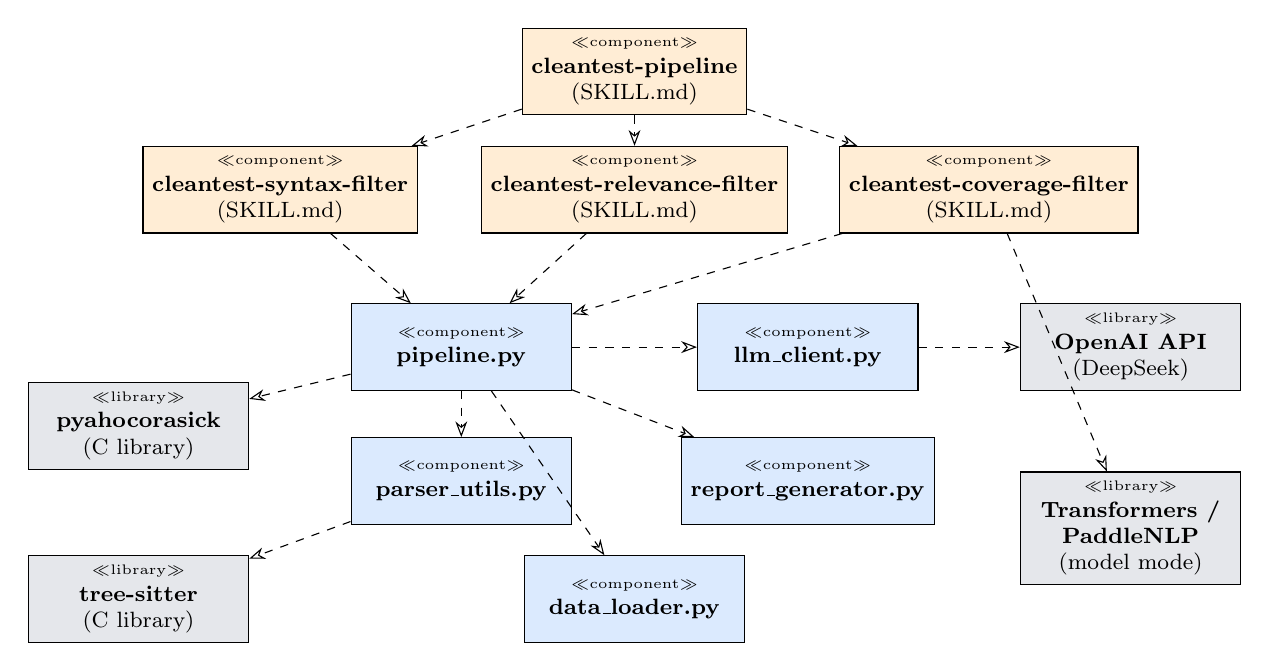
\begin{tikzpicture}[
    node distance=0.8cm,
    comp/.style={rectangle, draw, minimum width=2.8cm, minimum height=1.1cm,
                 align=center, font=\footnotesize, line width=0.4pt},
    % UML 2.5.1 §7.8.4 Dependency: dashed line with an open V-shaped
    % stick arrowhead (NOT a triangular arrowhead, which denotes
    % generalization or realization).
    dep/.style={-{Stealth[length=2mm,open]}, dashed, line width=0.4pt},
]
% --- Skills layer (UML 2.5.1 components are stereotyped <<component>>).
\node[comp, fill=cSkill] (pipe) at (0,4)
    {{\tiny$\ll$component$\gg$}\\\textbf{cleantest-pipeline}\\(SKILL.md)};
\node[comp, fill=cSkill] (sf) at (-4.5,2.5)
    {{\tiny$\ll$component$\gg$}\\\textbf{cleantest-syntax-filter}\\(SKILL.md)};
\node[comp, fill=cSkill] (rf) at (0,2.5)
    {{\tiny$\ll$component$\gg$}\\\textbf{cleantest-relevance-filter}\\(SKILL.md)};
\node[comp, fill=cSkill] (cf) at (4.5,2.5)
    {{\tiny$\ll$component$\gg$}\\\textbf{cleantest-coverage-filter}\\(SKILL.md)};

% --- Core library
\node[comp, fill=cCore] (pipeline) at (-2.2,0.5)
    {{\tiny$\ll$component$\gg$}\\\textbf{pipeline.py}};
\node[comp, fill=cCore] (parser) at (-2.2,-1.2)
    {{\tiny$\ll$component$\gg$}\\\textbf{parser\_utils.py}};
\node[comp, fill=cCore] (llm) at (2.2,0.5)
    {{\tiny$\ll$component$\gg$}\\\textbf{llm\_client.py}};
\node[comp, fill=cCore] (report) at (2.2,-1.2)
    {{\tiny$\ll$component$\gg$}\\\textbf{report\_generator.py}};
\node[comp, fill=cCore] (loader) at (0,-2.7)
    {{\tiny$\ll$component$\gg$}\\\textbf{data\_loader.py}};

% --- External libraries (custom <<library>> stereotype).
\node[comp, fill=cLib] (ts) at (-6.3,-2.7)
    {{\tiny$\ll$library$\gg$}\\\textbf{tree-sitter}\\(C library)};
\node[comp, fill=cLib] (aho) at (-6.3,-0.5)
    {{\tiny$\ll$library$\gg$}\\\textbf{pyahocorasick}\\(C library)};
\node[comp, fill=cLib] (api) at (6.3,0.5)
    {{\tiny$\ll$library$\gg$}\\\textbf{OpenAI API}\\(DeepSeek)};
\node[comp, fill=cLib] (tf) at (6.3,-1.8)
    {{\tiny$\ll$library$\gg$}\\\textbf{Transformers /}\\\textbf{PaddleNLP}\\(model mode)};

% --- Dependencies (UML 2.5.1 §7.8.4: dashed line + open V arrowhead).
\draw[dep] (pipe) -- (sf);
\draw[dep] (pipe) -- (rf);
\draw[dep] (pipe) -- (cf);
\draw[dep] (sf) -- (pipeline);
\draw[dep] (rf) -- (pipeline);
\draw[dep] (cf) -- (pipeline);
\draw[dep] (pipeline) -- (parser);
\draw[dep] (pipeline) -- (llm);
\draw[dep] (pipeline) -- (report);
\draw[dep] (pipeline) -- (loader);
\draw[dep] (parser) -- (ts);
\draw[dep] (pipeline) -- (aho);
\draw[dep] (llm) -- (api);
\draw[dep] (cf) -- (tf);
\end{tikzpicture}
\end{document}
"   % grayscale
%
% Or use the wrapper script:
%     ./build-figures.sh
%
% Notes on classfile choice:
%     We use `article` + `geometry` (everywhere available) instead of
%     `standalone` (requires `texlive-pictures`, not in BasicTeX) so the
%     figure builds on a stripped-down TeX install. The generated PDF is
%     subsequently cropped to the figure bounding box by `pdfcrop`,
%     yielding the same artefact a `standalone` build would.
% =====================================================================
\documentclass[11pt]{article}

\usepackage[paperwidth=22cm,paperheight=8.8cm,margin=4mm]{geometry}
\usepackage{lmodern}            % Computer Modern at scalable Type-1
\usepackage[T1]{fontenc}
\usepackage{tikz}
\usetikzlibrary{shapes,arrows.meta,positioning,calc}
\pagestyle{empty}

% ---------------------------------------------------------------------
% \BW = 1 switches to a print-safe grayscale palette. Default is the
% colour palette used in the paper (orange skills / blue core / grey
% libraries), which is the convention this figure has in the report.
% ---------------------------------------------------------------------
\providecommand{\BW}{0}

\ifnum\BW=1
  \definecolor{cSkill}{gray}{0.92}
  \definecolor{cCore} {gray}{0.85}
  \definecolor{cLib}  {gray}{0.78}
\else
  \definecolor{cSkill}{RGB}{255,237,213}   % orange!10
  \definecolor{cCore} {RGB}{219,234,254}   % blue!10
  \definecolor{cLib}  {RGB}{229,231,235}   % gray!10
\fi

\begin{document}
\centering
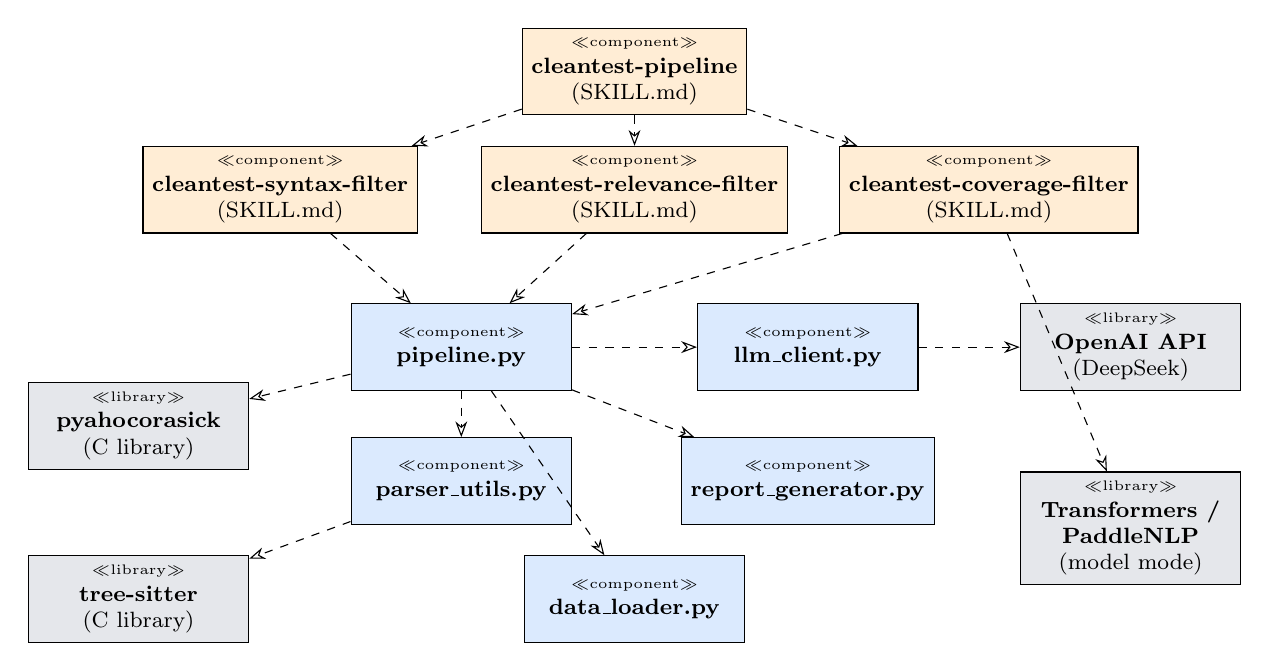
\begin{tikzpicture}[
    node distance=0.8cm,
    comp/.style={rectangle, draw, minimum width=2.8cm, minimum height=1.1cm,
                 align=center, font=\footnotesize, line width=0.4pt},
    % UML 2.5.1 §7.8.4 Dependency: dashed line with an open V-shaped
    % stick arrowhead (NOT a triangular arrowhead, which denotes
    % generalization or realization).
    dep/.style={-{Stealth[length=2mm,open]}, dashed, line width=0.4pt},
]
% --- Skills layer (UML 2.5.1 components are stereotyped <<component>>).
\node[comp, fill=cSkill] (pipe) at (0,4)
    {{\tiny$\ll$component$\gg$}\\\textbf{cleantest-pipeline}\\(SKILL.md)};
\node[comp, fill=cSkill] (sf) at (-4.5,2.5)
    {{\tiny$\ll$component$\gg$}\\\textbf{cleantest-syntax-filter}\\(SKILL.md)};
\node[comp, fill=cSkill] (rf) at (0,2.5)
    {{\tiny$\ll$component$\gg$}\\\textbf{cleantest-relevance-filter}\\(SKILL.md)};
\node[comp, fill=cSkill] (cf) at (4.5,2.5)
    {{\tiny$\ll$component$\gg$}\\\textbf{cleantest-coverage-filter}\\(SKILL.md)};

% --- Core library
\node[comp, fill=cCore] (pipeline) at (-2.2,0.5)
    {{\tiny$\ll$component$\gg$}\\\textbf{pipeline.py}};
\node[comp, fill=cCore] (parser) at (-2.2,-1.2)
    {{\tiny$\ll$component$\gg$}\\\textbf{parser\_utils.py}};
\node[comp, fill=cCore] (llm) at (2.2,0.5)
    {{\tiny$\ll$component$\gg$}\\\textbf{llm\_client.py}};
\node[comp, fill=cCore] (report) at (2.2,-1.2)
    {{\tiny$\ll$component$\gg$}\\\textbf{report\_generator.py}};
\node[comp, fill=cCore] (loader) at (0,-2.7)
    {{\tiny$\ll$component$\gg$}\\\textbf{data\_loader.py}};

% --- External libraries (custom <<library>> stereotype).
\node[comp, fill=cLib] (ts) at (-6.3,-2.7)
    {{\tiny$\ll$library$\gg$}\\\textbf{tree-sitter}\\(C library)};
\node[comp, fill=cLib] (aho) at (-6.3,-0.5)
    {{\tiny$\ll$library$\gg$}\\\textbf{pyahocorasick}\\(C library)};
\node[comp, fill=cLib] (api) at (6.3,0.5)
    {{\tiny$\ll$library$\gg$}\\\textbf{OpenAI API}\\(DeepSeek)};
\node[comp, fill=cLib] (tf) at (6.3,-1.8)
    {{\tiny$\ll$library$\gg$}\\\textbf{Transformers /}\\\textbf{PaddleNLP}\\(model mode)};

% --- Dependencies (UML 2.5.1 §7.8.4: dashed line + open V arrowhead).
\draw[dep] (pipe) -- (sf);
\draw[dep] (pipe) -- (rf);
\draw[dep] (pipe) -- (cf);
\draw[dep] (sf) -- (pipeline);
\draw[dep] (rf) -- (pipeline);
\draw[dep] (cf) -- (pipeline);
\draw[dep] (pipeline) -- (parser);
\draw[dep] (pipeline) -- (llm);
\draw[dep] (pipeline) -- (report);
\draw[dep] (pipeline) -- (loader);
\draw[dep] (parser) -- (ts);
\draw[dep] (pipeline) -- (aho);
\draw[dep] (llm) -- (api);
\draw[dep] (cf) -- (tf);
\end{tikzpicture}
\end{document}
